\documentclass{article}[12pt]

\addtolength{\oddsidemargin}{-.75in}%
\addtolength{\evensidemargin}{-.75in}%
\addtolength{\textwidth}{1.5in}%
\addtolength{\textheight}{1.3in}%
\addtolength{\topmargin}{-.8in}%
\addtolength{\marginparpush}{-.75in}%
%\setlength\parindent{0pt}
%\setlength{\bibsep}{0pt plus 0.3ex}

\usepackage[authoryear]{natbib}
\usepackage{graphicx}
\usepackage{algorithm,algorithmic}

\title{Variational approximations for zero-inflated Semiparametric Regression models}
\author{Mark Greenaway}
% include.tex
\newcommand{\Bernoulli}[1]{\text{Bernoulli} \left( #1 \right)}
\newcommand{\mydigamma}[1]{\psi \left( #1 \right)}
%\newcommand{\diag}[1]{\text{diag}\left( #1 \right)}
\newcommand{\tr}[1]{\text{tr}\left( #1 \right)}
\newcommand{\Poisson}[1]{\text{Poisson} \left( #1 \right)}
\def \half {\frac{1}{2}}
\def \R {\mathbb{R}}
\def \vbeta {\vec{\beta}}
\def \vy {\vec{y}}
\def \vmu {\vec{\mu}}
\def \vmuqbeta {\vmu_{q(\vbeta)}}
\def \vmubeta {\vmu_{\vbeta}}
\def \Sigmaqbeta {\Sigma_{q(\vbeta)}}
\def \Sigmabeta {\Sigma_{\vbeta}}
\def \va {\vec{a}}
\def \vtheta {\vec{\theta}}
\def \mX {\vec{X}}

\def\ds{{\displaystyle}}

\def\diag{{\mbox{diag}}}


\usepackage{latexsym,amssymb,amsmath,amsfonts}
%\usepackage{tabularx}
\usepackage{theorem}
\usepackage{verbatim,array,multicol,palatino}
\usepackage{graphicx}
\usepackage{graphics}
\usepackage{fancyhdr}
\usepackage{algorithm,algorithmic}
\usepackage{url}
%\usepackage[all]{xy}



\def\approxdist{\stackrel{{\tiny \mbox{approx.}}}{\sim}}
\def\smhalf{\textstyle{\frac{1}{2}}}
\def\vxnew{\vx_{\mbox{{\tiny new}}}}
\def\bib{\vskip12pt\par\noindent\hangindent=1 true cm\hangafter=1}
\def\jump{\vskip3mm\noindent}
\def\etal{{\em et al.}}
\def\etahat{{\widehat\eta}}
\def\thick#1{\hbox{\rlap{$#1$}\kern0.25pt\rlap{$#1$}\kern0.25pt$#1$}}
\def\smbbeta{{\thick{\scriptstyle{\beta}}}}
\def\smbtheta{{\thick{\scriptstyle{\theta}}}}
\def\smbu{{\thick{\scriptstyle{\rm u}}}}
\def\smbzero{{\thick{\scriptstyle{0}}}}
\def\boxit#1{\begin{center}\fbox{#1}\end{center}}
\def\lboxit#1{\vbox{\hrule\hbox{\vrule\kern6pt
      \vbox{\kern6pt#1\kern6pt}\kern6pt\vrule}\hrule}}
\def\thickboxit#1{\vbox{{\hrule height 1mm}\hbox{{\vrule width 1mm}\kern6pt
          \vbox{\kern6pt#1\kern6pt}\kern6pt{\vrule width 1mm}}
               {\hrule height 1mm}}}


%\sloppy
%\usepackage{geometry}
%\geometry{verbose,a4paper,tmargin=20mm,bmargin=20mm,lmargin=40mm,rmargin=20mm}


%%%%%%%%%%%%%%%%%%%%%%%%%%%%%%%%%%%%%%%%%%%%%%%%%%%%%%%%%%%%%%%%%%%%%%%%%%%%%%%%
%
% Some convenience definitions
%
% \bf      -> vector
% \sf      -> matrix
% \mathcal -> sets or statistical
% \mathbb  -> fields or statistical
%
%%%%%%%%%%%%%%%%%%%%%%%%%%%%%%%%%%%%%%%%%%%%%%%%%%%%%%%%%%%%%%%%%%%%%%%%%%%%%%%%

% Sets or statistical values
\def\sI{{\mathcal I}}                            % Current Index set
\def\sJ{{\mathcal J}}                            % Select Index set
\def\sL{{\mathcal L}}                            % Likelihood
\def\sl{{\ell}}                                  % Log-likelihood
\def\sN{{\mathcal N}}                            
\def\sS{{\mathcal S}}                            
\def\sP{{\mathcal P}}                            
\def\sQ{{\mathcal Q}}                            
\def\sB{{\mathcal B}}                            
\def\sD{{\mathcal D}}                            
\def\sT{{\mathcal T}}
\def\sE{{\mathcal E}}                            
\def\sF{{\mathcal F}}                            
\def\sC{{\mathcal C}}                            
\def\sO{{\mathcal O}}                            
\def\sH{{\mathcal H}} 
\def\sR{{\mathcal R}}                            
\def\sJ{{\mathcal J}}                            
\def\sCP{{\mathcal CP}}                            
\def\sX{{\mathcal X}}                            
\def\sA{{\mathcal A}} 
\def\sZ{{\mathcal Z}}                            
\def\sM{{\mathcal M}}                            
\def\sK{{\mathcal K}}     
\def\sG{{\mathcal G}}                         
\def\sY{{\mathcal Y}}                         
\def\sU{{\mathcal U}}  


\def\sIG{{\mathcal IG}}                            


\def\cD{{\sf D}}
\def\cH{{\sf H}}
\def\cI{{\sf I}}

% Vectors
\def\vectorfontone{\bf}
\def\vectorfonttwo{\boldsymbol}
\def\va{{\vectorfontone a}}                      %
\def\vb{{\vectorfontone b}}                      %
\def\vc{{\vectorfontone c}}                      %
\def\vd{{\vectorfontone d}}                      %
\def\ve{{\vectorfontone e}}                      %
\def\vf{{\vectorfontone f}}                      %
\def\vg{{\vectorfontone g}}                      %
\def\vh{{\vectorfontone h}}                      %
\def\vi{{\vectorfontone i}}                      %
\def\vj{{\vectorfontone j}}                      %
\def\vk{{\vectorfontone k}}                      %
\def\vl{{\vectorfontone l}}                      %
\def\vm{{\vectorfontone m}}                      % number of basis functions
\def\vn{{\vectorfontone n}}                      % number of training samples
\def\vo{{\vectorfontone o}}                      %
\def\vp{{\vectorfontone p}}                      % number of unpenalized coefficients
\def\vq{{\vectorfontone q}}                      % number of penalized coefficients
\def\vr{{\vectorfontone r}}                      %
\def\vs{{\vectorfontone s}}                      %
\def\vt{{\vectorfontone t}}                      %
\def\vu{{\vectorfontone u}}                      % Penalized coefficients
\def\vv{{\vectorfontone v}}                      %
\def\vw{{\vectorfontone w}}                      %
\def\vx{{\vectorfontone x}}                      % Covariates/Predictors
\def\vy{{\vectorfontone y}}                      % Targets/Labels
\def\vz{{\vectorfontone z}}                      %

\def\vone{{\vectorfontone 1}}
\def\vzero{{\vectorfontone 0}}

\def\valpha{{\vectorfonttwo \alpha}}             %
\def\vbeta{{\vectorfonttwo \beta}}               % Unpenalized coefficients
\def\vgamma{{\vectorfonttwo \gamma}}             %
\def\vdelta{{\vectorfonttwo \delta}}             %
\def\vepsilon{{\vectorfonttwo \epsilon}}         %
\def\vvarepsilon{{\vectorfonttwo \varepsilon}}   % Vector of errors
\def\vzeta{{\vectorfonttwo \zeta}}               %
\def\veta{{\vectorfonttwo \eta}}                 % Vector of natural parameters
\def\vtheta{{\vectorfonttwo \theta}}             % Vector of combined coefficients
\def\vvartheta{{\vectorfonttwo \vartheta}}       %
\def\viota{{\vectorfonttwo \iota}}               %
\def\vkappa{{\vectorfonttwo \kappa}}             %
\def\vlambda{{\vectorfonttwo \lambda}}           % Vector of smoothing parameters
\def\vmu{{\vectorfonttwo \mu}}                   % Vector of means
\def\vnu{{\vectorfonttwo \nu}}                   %
\def\vxi{{\vectorfonttwo \xi}}                   %
\def\vpi{{\vectorfonttwo \pi}}                   %
\def\vvarpi{{\vectorfonttwo \varpi}}             %
\def\vrho{{\vectorfonttwo \rho}}                 %
\def\vvarrho{{\vectorfonttwo \varrho}}           %
\def\vsigma{{\vectorfonttwo \sigma}}             %
\def\vvarsigma{{\vectorfonttwo \varsigma}}       %
\def\vtau{{\vectorfonttwo \tau}}                 %
\def\vupsilon{{\vectorfonttwo \upsilon}}         %
\def\vphi{{\vectorfonttwo \phi}}                 %
\def\vvarphi{{\vectorfonttwo \varphi}}           %
\def\vchi{{\vectorfonttwo \chi}}                 %
\def\vpsi{{\vectorfonttwo \psi}}                 %
\def\vomega{{\vectorfonttwo \omega}}             %


% Matrices
%\def\matrixfontone{\sf}
%\def\matrixfonttwo{\sf}
\def\matrixfontone{\bf}
\def\matrixfonttwo{\boldsymbol}
\def\mA{{\matrixfontone A}}                      %
\def\mB{{\matrixfontone B}}                      %
\def\mC{{\matrixfontone C}}                      % Combined Design Matrix
\def\mD{{\matrixfontone D}}                      % Penalty Matrix for \vu_J
\def\mE{{\matrixfontone E}}                      %
\def\mF{{\matrixfontone F}}                      %
\def\mG{{\matrixfontone G}}                      % Penalty Matrix for \vu
\def\mH{{\matrixfontone H}}                      %
\def\mI{{\matrixfontone I}}                      % Identity Matrix
\def\mJ{{\matrixfontone J}}                      %
\def\mK{{\matrixfontone K}}                      %
\def\mL{{\matrixfontone L}}                      % Lower bound
\def\mM{{\matrixfontone M}}                      %
\def\mN{{\matrixfontone N}}                      %
\def\mO{{\matrixfontone O}}                      %
\def\mP{{\matrixfontone P}}                      %
\def\mQ{{\matrixfontone Q}}                      %
\def\mR{{\matrixfontone R}}                      %
\def\mS{{\matrixfontone S}}                      %
\def\mT{{\matrixfontone T}}                      %
\def\mU{{\matrixfontone U}}                      % Upper bound
\def\mV{{\matrixfontone V}}                      %
\def\mW{{\matrixfontone W}}                      % Variance Matrix i.e. diag(b'')
\def\mX{{\matrixfontone X}}                      % Unpenalized Design Matrix/Nullspace Matrix
\def\mY{{\matrixfontone Y}}                      %
\def\mZ{{\matrixfontone Z}}                      % Penalized Design Matrix/Kernel Space Matrix

\def\mGamma{{\matrixfonttwo \Gamma}}             %
\def\mDelta{{\matrixfonttwo \Delta}}             %
\def\mTheta{{\matrixfonttwo \Theta}}             %
\def\mLambda{{\matrixfonttwo \Lambda}}           % Penalty Matrix for \vnu
\def\mXi{{\matrixfonttwo \Xi}}                   %
\def\mPi{{\matrixfonttwo \Pi}}                   %
\def\mSigma{{\matrixfonttwo \Sigma}}             %
\def\mUpsilon{{\matrixfonttwo \Upsilon}}         %
\def\mPhi{{\matrixfonttwo \Phi}}                 %
\def\mOmega{{\matrixfonttwo \Omega}}             %
\def\mPsi{{\matrixfonttwo \Psi}}                 %

\def\mone{{\matrixfontone 1}}
\def\mzero{{\matrixfontone 0}}

% Fields or Statistical
\def\bE{{\mathbb E}}                             % Expectation
\def\bP{{\mathbb P}}                             % Probability
\def\bR{{\mathbb R}}                             % Reals
\def\bI{{\mathbb I}}                             % Reals
\def\bV{{\mathbb V}}                             % Reals

\def\vX{{\vectorfontone X}}                      % Targets/Labels
\def\vY{{\vectorfontone Y}}                      % Targets/Labels
\def\vZ{{\vectorfontone Z}}                      %

% Other
\def\etal{{\em et al.}}
\def\ds{\displaystyle}
\def\d{\partial}
\def\diag{\text{diag}}
%\def\span{\text{span}}
\def\blockdiag{\text{blockdiag}}
\def\tr{\text{tr}}
\def\RSS{\text{RSS}}
\def\df{\text{df}}
\def\GCV{\text{GCV}}
\def\AIC{\text{AIC}}
\def\MLC{\text{MLC}}
\def\mAIC{\text{mAIC}}
\def\cAIC{\text{cAIC}}
\def\rank{\text{rank}}
\def\MASE{\text{MASE}}
\def\SMSE{\text{SASE}}
\def\sign{\text{sign}}
\def\card{\text{card}}
\def\notexp{\text{notexp}}
\def\ASE{\text{ASE}}
\def\ML{\text{ML}}
\def\nullity{\text{nullity}}

\def\logexpit{\text{logexpit}}
\def\logit{\mbox{logit}}
\def\dg{\mbox{dg}}

\def\Bern{\mbox{Bernoulli}}
\def\sBernoulli{\mbox{Bernoulli}}
\def\sGamma{\mbox{Gamma}}
\def\sInvN{\mbox{Inv}\sN}
\def\sNegBin{\sN\sB}

\def\dGamma{\mbox{Gamma}}
\def\dInvGam{\mbox{Inv}\Gamma}

\def\Cov{\mbox{Cov}}
\def\Mgf{\mbox{Mgf}}

\def\mis{{mis}} 
\def\obs{{obs}}

\def\argmax{\operatornamewithlimits{\text{argmax}}}
\def\argmin{\operatornamewithlimits{\text{argmin}}}
\def\argsup{\operatornamewithlimits{\text{argsup}}}
\def\arginf{\operatornamewithlimits{\text{arginf}}}


\def\minimize{\operatornamewithlimits{\text{minimize}}}
\def\maximize{\operatornamewithlimits{\text{maximize}}}
\def\suchthat{\text{such that}}


\def\relstack#1#2{\mathop{#1}\limits_{#2}}
\def\sfrac#1#2{{\textstyle{\frac{#1}{#2}}}}


\def\comment#1{
\vspace{0.5cm}
\noindent \begin{tabular}{|p{14cm}|}  
\hline #1 \\ 
\hline 
\end{tabular}
\vspace{0.5cm}
}


\def\mytext#1{\begin{tabular}{p{13cm}}#1\end{tabular}}
\def\mytextB#1{\begin{tabular}{p{7.5cm}}#1\end{tabular}}
\def\mytextC#1{\begin{tabular}{p{12cm}}#1\end{tabular}}

\def\jump{\vskip3mm\noindent}

\def\KL{\text{KL}}
\def\N{\text{N}}
\def\Var{\text{Var}}

\def \E {\mathbb{E}}
\def \BigO {\text{O}}
\def \IG {\text{IG}}
\def \Beta {\text{Beta}}


\begin{document}
\setlength{\parindent}{0pt}
\maketitle

Abstract:

Keywords: Approximate Bayesian inference ; mixed model ; Markov chain Monte Carlo ; Stan ; penalized splines .

\section{Introduction}
\label{sec:introduction}

% First, simplest zero-inflated count model to consider.
Count data with a large number of zero counts arises in many areas of
application, such as data arising from physical activity studies, 
insurance claims, hospital visits or defects in manufacturing processes.

While simple forms of these models are easy to fit with maximum likelihood techniques,
more general models incorporating random effects, splines and missing data typically
have no closed form solutions. Fitting these models is typically done with Monte Carlo
Markov Chain techniques, but these can be slow and prone to convergence problems. We
propose using Variational Bayes to fit close approximations to these models
using a deterministic algorithm which converges much more quickly.

% Cite prior publications in this area

In this paper, we build upon the earlier work of \cite{lambert1992},
\cite{Ghosh20061360} and \cite{VatsaWilson2014}.

In Section \ref{sec:introduction} we provide the framework for our approach. In
Section \ref{sec:methodology} we extend our approach to incorporate regression modelling
and random effects. In Section \ref{sec:algorithms} we present algorithms for fitting these models.
In Section \ref{sec:results} we show how our approach offers computational advantages
over existing approaches. In Section \ref{sec:application} we show an application of our
method to physical activity data. Appendices contain details of our variational lower bound
derivation.

\section{Methodology}\label{sec:methodology}

In this section we present a VB approach to a Bayesian zero-inflated Poisson model
for count data with extra zeroes. After introducing Bayesian zero-inflated models
and VB methodology we derive the VB factorised approximation to the full Bayesian
model. 

\subsection{Variational Bayesian inference}

Semiparametric mean field Variational Bayes is an approximate Bayesian inference method as detailed in
\cite{RohdeWand2015}. As can be seen from the following derivation, the log of the full likelihood bounds the 
lower bound above.

\begin{align*}
\log p(\vy) &= \log p(\vy) \int q(\vtheta) d \vtheta \\
&= \int q(\vtheta) \log \{ \frac{p(\vtheta, \vy) / q(\vtheta)}{p(\vtheta | \vy) / q(\vtheta)} \} d \vtheta \\
&= \int q(\vtheta) \log \frac{p(\vy, \vtheta)}{q(\vtheta)} d \vtheta +
	 \text{KL} \{ {q(\vtheta) || p(\vtheta|\vy)} \} % \\
%& \geq \int q(\vtheta) \log \frac{p(\vy, \vtheta)}{q(\vtheta)} d \vtheta
\end{align*}

The approximation is found by iteratively minimising the Kullback-Leibler divergence between the true 
posterior and an approximating distribution, and thus maximising the variational lower bound as defined in 
Equation \ref{eq:lower_bound_defn}.

\begin{equation}
\label{eq:lower_bound_defn}
\int q(\vtheta) \log \frac{p(\vy, \vtheta)}{q(\vtheta)} d \vtheta
\end{equation}

Thus the optimal approximation $q^*(\vtheta)$ is

$$
q^*(\vtheta) = \argmin_{q \in Q} \text{KL} \{ {q(\vtheta) || p(\vtheta|\vy)} \}.
$$

A common approach is to assume an approximation in a factorised form
$$q(\vtheta) = \Pi_{i=1}^M q(\theta_i).$$
The variational lower bound is maximised iteratively. On each iteration, the value of each parameter in the
model is calculated as the expectation of the full likelihood relative to the other parameters in the model, 
which is referred to as the mean field update:
$$q_i^*(\theta_i) \propto \exp{\{ \bE_{-q(\theta_i)} \log p(\vy, \vtheta) \}}$$
This is done for each parameter in the model in turn.
This continues until the variational lower bound's increase is negligible and convergence is achieved.

\section{The zero-inflated Poisson regression model}

Variational approximations are well-suited to accelerating the fit of Bayesian zero-inflated models
to data. Typically zero-inflated models arise in applications where we wish to build multivariate regression 
models. To be able to construct multivariate models with as much generality as possible, we specify the full
model as a General Design Bayesian Generalized Linear Mixed Model, as in \citep{zhao06}. This allows us to 
incorporate within-subject correlation, measurement error, missing data and smoothing splines in our models.

% TODO: Lower bound graph
% TODO: Accuracy of approximations
% TODO: Application, physical activity data
% Random intercept, longitudinal data
% Graph demonstrating additional zeroes

% Idea: We can use an approximation of the from q(\beta, \u, \Sigma) q(\rho) \Product q(r_i)
% and use GVA on q(\beta, \u, \Sigma) and mean field updates on \rho and r_i

\subsection{Model}
Let $\mR = \diag{(\vr)}$. Let $\mC = [\mX \mZ], \vnu = [\vbeta^\top \vu^\top]^\top$. Consider the
model

$$
\begin{array}{rl}
\log{p(\vy|\vr, \vbeta, \vu)} &= \vy^\top \mR (\mC\vnu) - \vr^\top \exp{(\mC\vnu)} - \vone^\top \log{\Gamma{(\vy + \vone)}}, \\
\mbox{ and }
r_i &\sim \text{Bernoulli}(\rho) \\
\end{array}
$$

with priors

$$ 
\begin{array}{rl}
\log{p(\mSigma_{\vu \vu})} &= \text{Inverse Wishart}(\mPsi, v),\\
p(\rho) &\propto 1 \\
\mbox{ and } \vnu|\sigma_\vu^2 &\sim \mbox{N}(\vzero, \sigma_\vu^2). \\
\end{array}
$$

\subsection{Approximation}
Let $\vr_0 = \{ r_i : y_i = 0 \}$.
We assume an approximation of the form
$$
q(\vr_0, \vnu, \sigma_{\vu}^2, \rho) = q(\vnu) q(\mSigma_{\vu \vu}) q(\rho) q(\vr_0) \\
$$

where 
$q(\sigma_{\vu}^2) = \mbox{Inverse Wishart}\left(\mPsi + \sum_{i=1}^m \vmu_i \vmu_i^\top + \mLambda_{\vu_i \vu_i}, v + m + d\right)$ \mbox{and } $q(r_i) = \Bernoulli{(p_i)}$

with
$$
p_i = \expit\left[ \psi{(\alpha_{q(\rho)})} - \psi{(\beta_{q(\rho)})} - \exp{(c_i^\top\vmu + \half c_i^\top \mLambda c_i)} \right]
$$

\text{when} $\vy_i = 0$.

% What on Earth is this section doing here? This is very random.
%$\propto \exp{\left \{-r_i \bE_{-r_i} [\exp{(c_i^\top\vnu)}] + r_i [\psi(\alpha_\rho) - \psi(\beta_\rho)] \right \} }.\\$

% Include derivations for mean field updates at the end?

The optimal approximation for $\vr$ is
$$
\begin{array}{rl}
q(\vr) &\propto \exp \left [ \bE_{-q(\vr)}\vy^\top\mR(\mC\vmu) - \vr^\top\exp{(\mC\vnu)}-\half \vnu^\top \mSigma_{\vu \vu} \vnu \right ] \\ [1ex]
	&= \exp{ \left\{ \vy^\top\mR\mC \vmu - \vr^\top \exp{[\mC \vmu + \half \text{diag}(\mC \mLambda \mC^\top)]} - \half \vmu^\top \mD \vmu - \half \text{tr}(\mLambda \mD ) \right\} }
\end{array}
$$

where $\mD =  \left[ (\mPsi + \sum_{i=1}^m \vmu_i \vmu_i^\top + \mLambda_{\vu_i\vu_i}) / (v - d - 1) \right]^{-1}$. 

This is close in form to a Poisson regression model. Poisson regression models
with normal priors have no closed form for their mean field updates due to
non-conjugacy, but can be fit using Gaussian Variational Approximation, as in
\citep{ormerod09}. The model can be fit using Algorithm \ref{alg:algorithm_one} below.

\begin{algorithm}
\caption[Algorithm 1]{Iterative scheme for obtaining the parameters in the
optimal densities $q^*(\vmu, \mLambda)$, $q^*(\mSigma_{\vu \vu})$ and $q^*(\rho)$}
\label{alg:algorithm_one}
\begin{algorithmic}
% Fit \vmu, \mLambda using Laplace approximation
\REQUIRE{$\alpha_{q(\rho)} \leftarrow \alpha_\rho + \vone^\top\vp, p_{q(\mSigma_{\vu \vu})} \leftarrow p + 1$} \\[1ex]
\WHILE{the increase in $\log{\underline{p}}(\vy;q)$ is significant}
% \vmu, \mLambda
\STATE Optimise $\vmu$ and $\mLambda$ using $\vy, \mC, \vp$ and $\mSigma_{\vu \vu}$ \\[1ex]
% \vp
% \rho is a prior? Not directly observed, except through \vr_i
\STATE $\beta_{q(\rho)} \leftarrow \beta_\rho + n - \vone^\top\vp$ \\[1ex]
\STATE $\eta \leftarrow -\exp \left [ \mC \vmu + \half \diag{(\mC\mLambda\mC^\top)} \right ] + \psi{(\alpha_{q{(\rho)}})} - \psi{(\beta_{q{(\rho)}})}$ \\[1ex]
\STATE $\vp_{q(\vr_0)} \leftarrow \expit{(\eta)}$ \\[1ex]
% \mSigma_{\vu \vu}
\STATE $\mPsi_{q(\mSigma_{\vu \vu})} \leftarrow \Psi + \sum_{i=1}^m \vmu_i \vmu_i^\top + \mLambda_{{\vu}_i}$ \\[1ex]
\STATE $\mSigma_{\vu\vu} \leftarrow [\mPsi_{q(\mSigma_{\vu \vu})}/(v - d - 1)]^{-1}$
\ENDWHILE
\end{algorithmic}
\end{algorithm}

\section{Model fitting algorithms}
\label{sec:algorithms}

In this section, we compare the accuracy, stability and speed of a number of algorithms for fitting the 
variational approximation to our model.

\subsection{Laplace-Variational Approximation}
Laplace's method of approximation uses the second order Taylor expansion of the
full log likelihood around the mode to find a Gaussian approximation to the full posterior.
This can then be optimised using Newton-Raphson style iterations. The algorithm is very
quick to execute, but the resulting approximate posterior distributions are not as accurate
as those produced by the other algorithms considered in this article.

% NR
% Detail the function and its derivatives
Taylor expanding the full log likelihood once around the mode yields the following function
\begin{align*}
\log \underline{p}(\vmu, \mLambda; \vy) = \vy^\top\mP\mC\vmu - \vp^\top\exp \left (\mC \vmu \right ) - \half \vmu^\top \mSigma^{-1} \vmu.
\end{align*}

This can be optimised using a Newton-Raphson style algorithm where

\begin{align*}
\frac{\partial \log p(\vmu, \mLambda; \vy)}{\partial \vmu} &\approx \mP \mC (\vy - \exp{(\mC \vmu)}) - \mSigma^{-1} \vmu \text{ and} \\
\frac{\partial \log p(\vmu, \mLambda; \vy)}{\partial \mLambda} &\approx - \mC^\top \text{diag}(\vp e^{(\mC \vmu)}) \mC - \mSigma^{-1}.
\end{align*}

The steps of the algorithm are shown in Algorithm \ref{alg:laplace_alg}.

\begin{algorithm}
\caption{Laplace scheme for optimising $\log \underline{p}(\vmu, \mLambda; \vy)$}
\label{alg:laplace_alg}
\begin{algorithmic}
% Fit \vmu, \mLambda using Laplace approximation
\WHILE{the increase in $\log \underline{p}(\vmu, \mLambda; \vy)$ is significant}
% \vmu, \mLambda
\STATE $\mLambda \leftarrow \left [\mP \mC^\top \text{diag}(\exp{(\mC \vmu)}) \mC + \mSigma^{-1} \right ]^{-1}$ \\ [1ex] 
\STATE $\vmu \leftarrow \vmu + \mLambda \left [ \frac{\partial \log p(\vmu, \mLambda; \vy)}{\partial \vmu}  \right ]$ \\ [1ex]
\ENDWHILE
\end{algorithmic}
\end{algorithm}

\subsection{Optimising the GVA lower bound}
% Detail techniques used for fitting models.
% TODO: Talk more about numerical scheme. This explanation is terrible!
Assuming $q(\vnu) \sim N(\vmu, \mLambda)$, the Gaussian variational lower bound in Algorithm
\ref{alg:algorithm_one} can be optimised using a  variety of algorithms. The variational lower bound is not 
necessarily unimodal, leading to potential difficulty in optimising to the global maximum. However, for fixed
$\vp$ and $\mSigma$, the variational lower bound is log-concave, and so standard
optimisation methods such as L-BFGS-B work well. This led to an extremely accurate approximation
of the true posterior at the expense of some additional computational effort.

\subsubsection{GVA, $\mLambda = \mR \mR^\top$}
% TODO: Should talk about the reasons for choosing the various parameterisations
% Ensure positive definiteness of \mLambda

The first variant of the Gaussian Variational Approximation algorithm
optimises the Gaussian variational lower bound of the log likelihood with
respect to $\vmu$ and the Cholesky decomposition $\mR$ of $\mLambda$, that is,
$\mLambda = \mR \mR^\top$. This algorithm trades the computational complexity of
numerically evaluating an integral for greatly increased accuracy in the
approximating posterior distribution. The resulting function is below and  can
be optimised with L-BFGS-B

% Detail the function and its derivatives
\begin{align*}
\log \underline{p}(\vmu, \mLambda; \vy) &= \quad \vy^\top\mP \mC \vmu - \vp^\top \exp(\mC \vmu + \half \text{diag}(\mC \mLambda \mC^\top)) - \half \vmu^\top \mSigma^{-1} \vmu - \half \tr{(\mSigma^{-1} \mLambda)} + \log{|\mR|} \\
&\quad - \frac{d}{2} \log{(2 \pi)} + \half \log{|\mSigma^{-1}|} + \frac{d}{2} \log{(2 \pi)} + \frac{d}{2} \\
\end{align*}

using the derivatives

\begin{align*}
\frac{\partial \log \underline{p}(\vmu, \mLambda; \vy)}{\partial \vmu} &= \mP \mC (\vy - \mC^\top \exp(\mC \vmu + \half \text{diag}{(\mC \mLambda \mC^\top)})) - \mSigma^{-1} \vmu \text{ and}\\
\frac{\partial \log \underline{p}(\vmu, \mLambda; \vy)}{\partial \mLambda} &= \left [\mLambda^{-1} - \mP \mC^\top \exp(\mC \vmu + \half \text{diag}(\mC \mLambda \mC^\top)) \mP \mC) - \mSigma^{-1} \right ] \mR.
\end{align*}

\subsubsection{GVA, $\mLambda = \left (\mR \mR^\top \right )^{-1}$}
The second variant of the Gaussian Variational Approximation algorithm is similiar 
to the first, but instead of optimising the Gaussian variational lower bound with respect to
$\vmu$ and the Cholesky factor $\mR$ of $\mLambda$, we instead optimise the Cholesky factor of the inverse of
$\mLambda$ i.e. $\mLambda = (\mR \mR^\top)^{-1}$.

This new choice of parameterisation allows us to calculate $\exp(\mC \vmu + \half
\text{diag}(\mC \mLambda \mC^\top))$ and its derivatives by solving $\mR \va = \mC_{i},
 i=1, \ldots, n$ for $\va$ and then calculating $\va^\top\va$ rather than calculating
$\text{diag}(\mC \mLambda \mC^\top)$ directly.

By re-ordering $\mC = [\mX \mZ]$ to $\mC = [\mZ \mX]$, and re-ordering the dimensions
of $\vmu, \mLambda$ and $\mSigma$ in the same manner, the independence between the
blocks relating to the random effects in $\mZ$ induce sparsity in the Cholesky factor $\mR$
of $\mLambda$. Thus the Gaussian $q(\vnu) \sim N(\vmu, \mLambda)$ can be optimised over a space
of $\half p (p + 1) + pq + \half q (q + 1)$ rather than dimension $\half (p + mq) (p + mq + 1)$ 
as in the dense parameterisation. This leads to subtantial performance gains when m is large,
as is typically the case in problems of practical importance such as clinical trials or the application
presented in Section \ref{sec:application}.

The Gaussian variational lower bound in this parameterisation is

\begin{align*}
\log \underline{p}(\vmu, \mLambda; \vy) &= \quad \vy\mP\mC \vmu - \vp^\top \exp(\mC \vmu + \half \text{diag}(\mC \mLambda \mC^\top)) - \half \vmu^\top \mSigma^{-1} \vmu - \half \tr{(\mSigma^{-1} \mLambda)} \\
&\quad- \frac{d}{2} \log{(2 \pi)} + \half \log{|\mSigma^{-1}|} + \frac{d}{2} \log{(2 \pi)} + \frac{d}{2} - \log{|\mR|}
\end{align*}

The derivative with respect to $\vmu$ is the same as that in the GVA 
algorithm, but as the parameterisation of $\mLambda$ has changed, the  
derivative with respect to $\mLambda$ becomes

\begin{align*}
\partial \log \underline{p}(\vmu, \mLambda; \vy)/\partial \mLambda
&= \hphantom{-}(\mLambda^{-1} + \mH)(-\mLambda \mR \mLambda) \\
&= -(\mI + \mH\mLambda)\mR\mLambda \\
&= - (\mR\mLambda + \mH\mLambda\mR\mLambda)
\end{align*} 

where $\mH = (\mP \mC)^\top \text{diag}(\exp(\mC \vmu + \half \mC \mLambda \mC^\top)) \mP \mC - \mSigma^{-1}$.


\subsubsection{GVA fixed point}
% Fixed point update of \mLambda
This variant of the algorithm uses Newton-Raphson-like fixed point updates on the Gaussian
variational lower bound. This algorithm is fast, but unstable. The steps are presented in
Algorithm \ref{alg:algorithm_nr} where

\begin{align*}
\frac{\partial \log \underline{p}(\vmu, \mLambda; \vy)}{\partial \vmu} &= \quad \mC^\top\vp \left [\vy - \mC\exp(\mC \vmu + \half \text{diag}(\mC \mLambda \mC^\top)) \right ] - \mSigma^{-1} \vmu \text{ and}\\
\frac{\partial \log \underline{p}(\vmu, \mLambda; \vy)}{\partial \mLambda} &= -\mC^\top \text{diag}(\vp^\top \exp(\mC \vmu +\half \text{diag}(\mC \mLambda \mC^\top))) - \mSigma^{-1}.
\end{align*}

\begin{algorithm}
\caption[Algorithm GVA NR]{Iterative scheme for obtaining optimal $\vmu$ and $\mLambda$
given $\vy$, $\mC$ and $\vp$}
\label{alg:algorithm_nr}
\begin{algorithmic}
% Fit \vmu, \mLambda using Laplace approximation
\WHILE{the increase in $\log{\underline{p}}(\vmu, \mLambda; \vy)$ is significant}
% \vmu, \mLambda
\STATE $\mLambda \leftarrow \left [ \mP \mC^\top \exp(\mC \vmu + \half \text{diag}(\mC \mLambda \mC^\top)) \mC \right ]^{-1}$ \\ [1ex]
\STATE $\vmu \leftarrow \vmu + \mLambda \left [ \frac{\partial \log \underline{p}(\vmu, \mLambda; \vy)}{\partial \vmu} \right ]$
\ENDWHILE
\end{algorithmic}
\end{algorithm}

% Splines

\section{Results/Numerical experiments}
\label{sec:results}

The accuracy of each model fitting algorithm presented in Section \ref{sec:algorithms}} was assessed by comparing 
the approximating distribution of each parameter with the posterior distribution of Monte Carlo Markov Chain 
samples of that parameter. 1 million Monte Carlo Markov Chain samples were generated using Stan.

The results for the random intercept, random slope and spline accuracy are presented in
Table \ref{tab:accuracy_int}, Table \ref{tab:accuracy_slope} and Table \ref{tab:accuracy_spline}
respectively.

The stability of the algorithms was confirmed by running them on 10,000 
different data sets that were randomly generated after having initialised the random 
number generator with different seeds. Median accuracy of the algorithms was assessed
by running them on 100 randomly generated data sets.

% TODO - Graphs of median accuracy

% Table of accuracy results - intercept model
\begin{table}
\caption{Table of accuracy - Random intercept model}
\label{tab:accuracy_int}
\begin{tabular}{|l|cccc|}
\hline
& Laplace's Method & GVA $(\mLambda = \mR \mR^\top)$ & GVA2 $(\mLambda = (\mR \mR^\top)^{-1})$ & GVA FP\\
\hline
$\vbeta_1$ & $0.833$ & $0.908$ & $0.908$ & $0.908$ \\ 
$\vbeta_2$ & $0.770$ & $0.987$ & $0.987$ & $0.987$ \\ 
Mean of $\vu$ & $0.807$ & $0.947$ & $0.947$ & $0.947$ \\
$\sigma^2_{\vu_1}$ & $0.473$ & $0.471$ & $0.471$ & $0.471$ \\ 
$\rho$ & $0.976$ & $0.974$ & $0.974$ &  $0.974$ \\ 
\hline
\end{tabular}
\end{table}

\begin{table}
\caption{Table of accuracy - Random slope model}
\label{tab:accuracy_slope}
\begin{tabular}{|l|cccc|}
\hline
& Laplace's Method & GVA $(\mLambda = \mR \mR^\top)$ & GVA $(\mLambda = (\mR \mR^\top)^{-1})$ & GVA FP\\
\hline
$\vbeta_1$     &0.658&0.879&0.893&0.879\\
$\vbeta_2$     &0.692&0.883&0.899&0.883\\
Mean of $\vu$        &0.719&0.908&0.911&0.908\\
$\sigma^2_{\vu_1}$ &0.720&0.713&0.713&0.687\\
$\sigma^2_{\vu_2}$ &0.716&0.714&0.714&0.698\\
$\rho$ &0.911&0.896&0.896&0.896\\
\hline
\end{tabular}
\end{table}

% \begin{table}
% \caption{Table of accuracy - Splines}
% \label{tab:accuracy_spline}
% \begin{tabular}{|l|l|}
% \hline
% Approximation & Accuracy \\
% \hline
% Laplace's Method & 0.969 \\
% GVA & 0.969 \\
% GVA2 & 0.969 \\
% GVA NR & 0.969 \\
% \hline
% \end{tabular}
% \end{table}

\begin{figure}
\label{fig:spline}
\caption{Comparison of VB and MCMC spline fits with the true function}
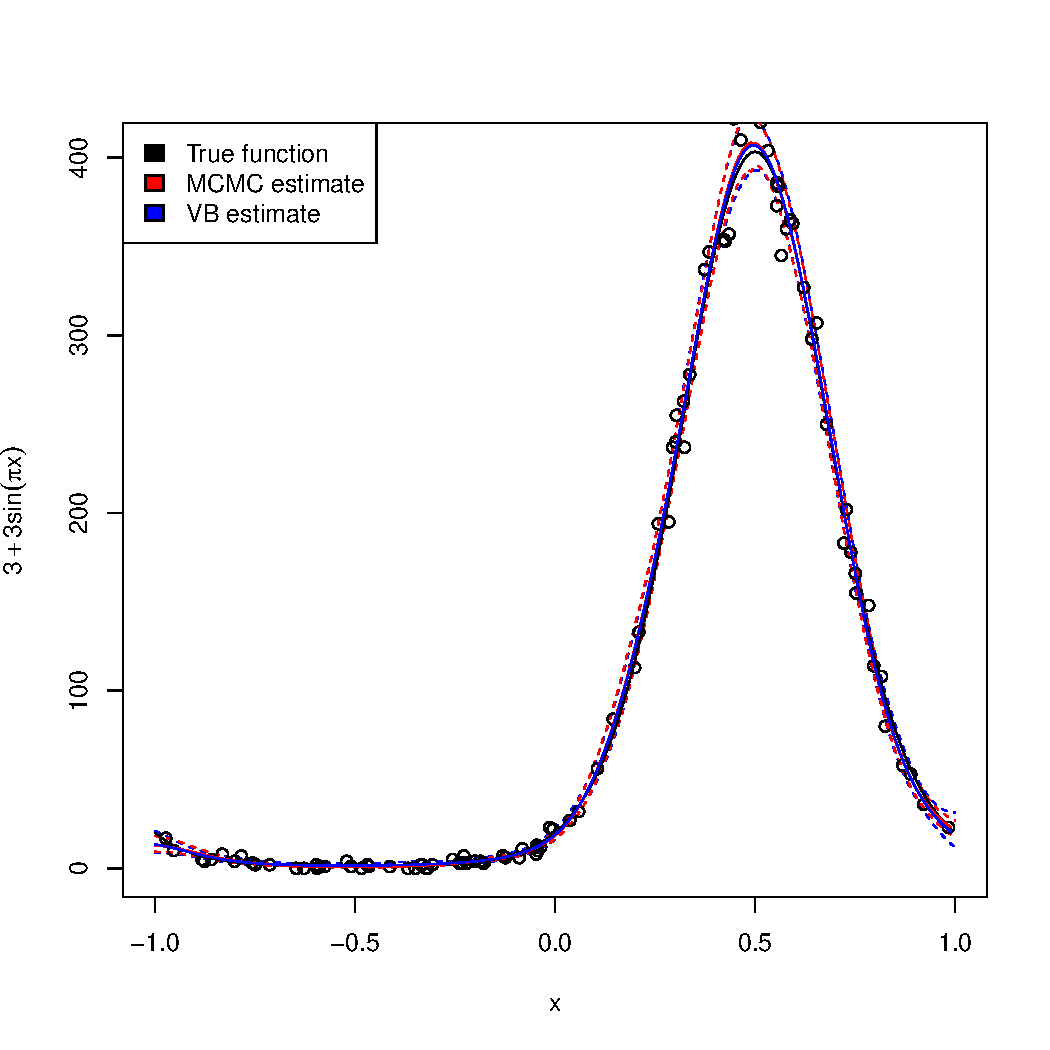
\includegraphics[width=100mm, height=100mm]{code/results/accuracy_plots_spline_gva2.pdf}
\end{figure}

% Graphs - exactly what sort of graphs do we need?
% Median accuracy
% Increase in lower bound
% MCMC posterior, with approximating posterior for at least one or two of the
% key parameters, such as, say, vbeta[2]

\subsection{Stability results}

The numerical stability of each fitting algorithm in Section \ref{sec:algorithms} was assessed by
initialising each algorithm from a range of different starting points. Errors due to numerical instability and 
the fitted $\vmu$ were recorded for each starting point.

A data set of 100 individuals in ten groups (m=10) was generated from a model with a fixed intercept and slope, 
and a random intercept. $\vmu$ was initialised from a grid of points on the interval $[-4.5, 5]$ for intercept 
and slope. The error counts are presented in Table \ref{tab:stability_results}.

\begin{table}
\caption{Count of numerical errors for each algorithm during stability tests}
\label{tab:stability_results}
\begin{tabular}{|l|l|}
\hline
Algorithm & Error \\
\hline
Laplace's algorithm & 9,216 \\
GVA & 1,771 \\
GVA2 & 776 \\
GVA FP & 992 \\
\hline
\end{tabular}
\end{table}

\section{Application}\label{sec:application}

The GVA2 algorithm was used to fit a random intercept model to the Roaches data set provided
by Andrew Gelman. The results are presented in Table \ref{tab:application_roaches}.

%              lci    uci
% 1   3.179  3.157  3.201
% 2  -0.046 -0.053 -0.039
% 3  -0.420 -0.434 -0.406
% 1  -0.976 -1.015 -0.936
% 2  -0.309 -0.323 -0.295
% 3  -0.947 -0.963 -0.930
% 4  -2.129 -2.384 -1.874
% 5  -3.230 -3.490 -2.970
% 6  -3.099 -3.404 -2.794
% 7  -1.290 -1.326 -1.255
% 8  -0.956 -0.991 -0.921
% 9  -2.404 -2.600 -2.209
% 10 -1.076 -1.123 -1.029
% 11 -1.079 -1.107 -1.052
% 12 -1.681 -1.737 -1.624

%> round(cbind(fit1$vmu, lci, uci), 3)
%  fit1$a_rho
% [1] 377.2375
% > fit1$b_rho
% [1] 152.7625

\begin{table}
\caption{Table of results - Roaches}
\label{tab:application_roaches}
\begin{tabular}{|l|llll|}
\hline
Covariate & Posterior Mean & Lower 95\% CI &  Upper 95\% CI & Accuracy \\
\hline
Intercept & 3.179 & 3.157 & 3.201 & 0.896 \\
Time & -0.046 & -0.053 & -0.039 & 0.965 \\
Time:Treatment & -0.428 & -0.434 & -0.406 & 0.929 \\
Random intercept & -1.600 & -1.705 & -1.491 & 0.895 \\
$\sigma^2_{\vu_1}$ & 0.577 & 0.574 & 0.574 & 0.574 \\
$\rho$ & 0.711 & 0.673 & 0.750 & 0.876 \\
\hline
\end{tabular}
\end{table}

% Figure: Median accuracy graph intercept
% Figure: Median accuracy graph slope

\newpage
\section{Appendix} 
% TODO: Mean field updates?
\subsection{Calculation of the Variational Lower bound}
% Where are the priors for \vbeta and \vu
The variational lower bound is equal to
$\bE_q[\log{p(\vy, \vtheta)} - \log{q(\vtheta)}] = T_1 + T_2 + T_3$,
where

% This is the new T_1
$$
\begin{array}{rl}
T_1 &= \quad \bE_q[\log{p(\vy, \vnu)} - \log{q(\vnu)}] \\
&= \quad \vy \mP \mC \vmu - \vp^\top \exp{\left[ \mC \vmu + \half \text{diag} (\mC \mLambda \mC^\top) \right]} - \vone^\top\log \Gamma{(\vy + \vone)}\\
& \quad + \frac{p + m}{2} (1 + \log{2 \pi}) + \half \log{|\mLambda|}, \\
T_2 &= \quad \bE_q \left[ \log p(\mSigma_{\vu \vu}) - \log q(\mSigma_{\vu \vu}) \right] \\
&= \quad \bE_q \big[ v/2(\log |\Psi| - \log |\Psi + \vmu_\vu \vmu_\vu^\top + \mLambda_{\vu \vu}|) + \half \log 2 + \half \log|\mSigma_{\vu \vu}| + \log \Gamma_{p+1}(v/2) - \log \Gamma_{p}(v/2)\\
&\quad + \half \tr((\vmu_{\vu} \vmu_{\vu}^\top + \mLambda_{\vu \vu}) \mSigma_{\vu \vu}^{-1}) \big] \\
&= \quad v/2\big(\log |\Psi| - \log |\Psi + \vmu_\vu \vmu_\vu^\top + \mLambda_{\vu \vu}|\big) + \half \log 2 + \half \bE_q \log |\mSigma_{\vu \vu}| + \log \Gamma_{p+1}(v/2) - \log \Gamma_{p}(v/2) \\
&\quad + \half \tr\big(\mI_m + \Psi(\Psi+ \vmu_\vu \vmu_\vu^\top + \mLambda_{\vu \vu})^{-1}/(v + p + 2)\big) \\
T_3 &= - \vp^\top \log \vp - (\vone - \vp)^\top \log (\vone - \vp) - \log \Beta (\alpha_\rho, \beta_\rho) + \log \Beta (\alpha_q, \beta_q)
\end{array}
$$

with $\bE_q \big[ \log |\mSigma_{\vu \vu}| \big] = m \log 2 + \log \left | \Psi + \vmu_\vu \vmu_\vu^\top + \mLambda_{\vu \vu} \right | + \sum_{i=1}^m \Psi \left ( \frac{v - i + 1}{2} \right )$

\bibliographystyle{elsarticle-harv}
\bibliography{Chapter_1_zero_inflated_models}

\end{document}
